\begin{figure}[H]
    \centering
    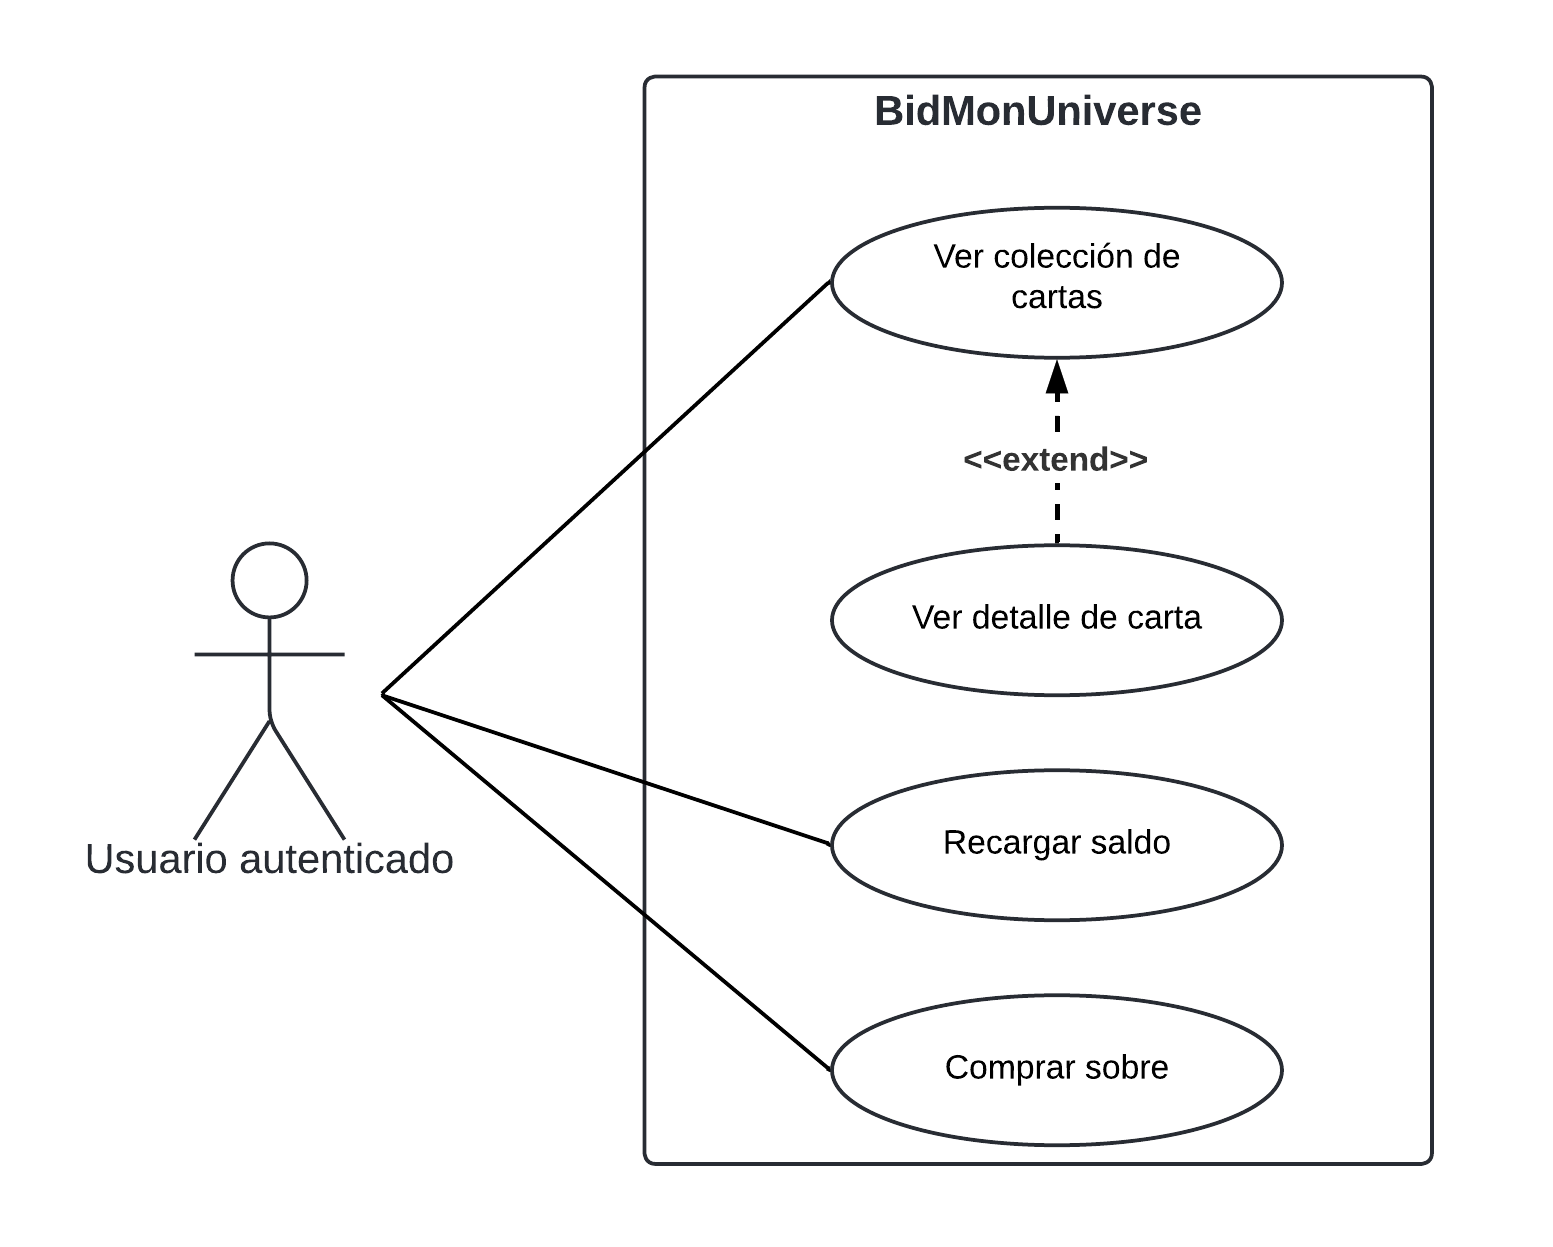
\includegraphics[width=0.5\textwidth]{figures/6-Analisis/6-Casos-uso/6_3_3_Gestion-coleccion-cartas.png}
    \caption{Casos de uso. Gestión de colección de cartas}
    \label{fig:cu_gestion-coleccion-cartas}
\end{figure}

\subsubsection{Caso de uso. Ver colección de cartas} \label{sec:cu_coleccion-cartas}
\begin{longtable}{
    >{\columncolor{lightgreen!20}}p{4cm}
    p{12cm}
    }
    \caption{Caso de uso. Ver colección de cartas} \label{table:cu_coleccion-cartas} \\
    \toprule
    \rowcolor{darkgreen!50}
    \textbf{Caso de uso} & \multicolumn{1}{>{\columncolor{darkgreen!50}\centering\arraybackslash}p{12cm}}{\textbf{VER COLECCIÓN DE CARTAS}} \\
    \endfirsthead
    
    \multicolumn{2}{c}%
    {{ \tablename\ \thetable{} Caso de uso. Ver colección de cartas -- continuación de la página anterior}} \\
    \toprule
    \rowcolor{darkgreen!50}
    \textbf{Caso de uso} & \multicolumn{1}{>{\columncolor{darkgreen!50}\centering\arraybackslash}p{12cm}}{\textbf{VER COLECCIÓN DE CARTAS}} \\
    \midrule
    \endhead
    
    \midrule
    \multicolumn{2}{r}{{Continúa en la siguiente página...}} \\ 
    \endfoot
    
    \bottomrule
    \endlastfoot
    
    \midrule
    Descripción & Un usuario autenticado puede ver la colección de cartas que posee. \\
    \midrule
    Actores principales & Usuario autenticado \\
    \midrule
    Actores secundarios &  \\
    \midrule
    Precondiciones & \begin{itemize}[nosep,leftmargin=*]
        \item El usuario debe haber iniciado sesión en el sistema.
    \end{itemize} \\
    \midrule
    Postcondiciones & \\
    \midrule
    Disparadores & El usuario accede a la sección de colección de cartas. \\
    \midrule
    Escenario principal & \begin{enumerate}[nosep,leftmargin=*]
        \item El sistema muestra la colección de cartas del usuario.
    \end{enumerate} \\
    \midrule
    Escenarios alternativos & 
    \begin{itemize}[nosep,leftmargin=*]
        \item \textbf{Escenario alternativo 1. El usuario no tiene cartas en su colección.}
        \begin{enumerate}[nosep,leftmargin=*]
            \item Se mostrará un mensaje indicando que el usuario no tiene cartas en su colección.
            \item Se mostrará la opción de comprar un sobre de cartas.
        \end{enumerate}
    \end{itemize} \\
    \midrule
    Situaciones de error & 
    \begin{itemize}[nosep,leftmargin=*]
        \item \textbf{Error de conexión a la base de datos.}
        \begin{enumerate}[nosep,leftmargin=*]
            \item El sistema mostrará un mensaje de error.
            \item El sistema le dará al usuario la opción de volver a la página principal.
        \end{enumerate}
    \end{itemize} \\
\end{longtable}

\subsubsection{Caso de uso. Ver detalle de una carta} \label{sec:cu_detalle-carta}
\begin{longtable}{
    >{\columncolor{lightgreen!20}}p{4cm}
    p{12cm}
    }
    \caption{Caso de uso. Ver detalle de una carta} \label{table:cu_detalle-carta} \\
    \toprule
    \rowcolor{darkgreen!50}
    \textbf{Caso de uso} & \multicolumn{1}{>{\columncolor{darkgreen!50}\centering\arraybackslash}p{12cm}}{\textbf{VER DETALLE DE UNA CARTA}} \\
    \endfirsthead
    
    \multicolumn{2}{c}%
    {{ \tablename\ \thetable{} Caso de uso. Ver detalle de una carta -- continuación de la página anterior}} \\
    \toprule
    \rowcolor{darkgreen!50}
    \textbf{Caso de uso} & \multicolumn{1}{>{\columncolor{darkgreen!50}\centering\arraybackslash}p{12cm}}{\textbf{VER DETALLE DE UNA CARTA}} \\
    \midrule
    \endhead
    
    \midrule
    \multicolumn{2}{r}{{Continúa en la siguiente página...}} \\ 
    \endfoot
    
    \bottomrule
    \endlastfoot
    
    \midrule
    Descripción & Un usuario autenticado puede ver el detalle de una carta de su colección. \\
    \midrule
    Actores principales & Usuario autenticado \\
    \midrule
    Actores secundarios &  \\
    \midrule
    Precondiciones & \begin{itemize}[nosep,leftmargin=*]
        \item El usuario debe haber iniciado sesión en el sistema.
    \end{itemize} \\
    \midrule
    Postcondiciones & \\
    \midrule
    Disparadores & El usuario accede a la sección de colección de cartas y selecciona una carta. \\
    \midrule
    Escenario principal & \begin{enumerate}[nosep,leftmargin=*]
        \item El sistema muestra la colección de cartas del usuario.
        \item El usuario puede seleccionar una carta para ver su información detallada.
        \item El sistema redirige al usuario a la página de detalle de la carta seleccionada.
        \item El usuario puede consultar la información detallada de la carta.
        \item El usuario puede consultar el histórico de transacciones de la carta.
        \item Si la carta no está en subasta, el usuario puede ponerla en subasta.
    \end{enumerate} \\
    \midrule
    Escenarios alternativos &  \\
    \midrule
    Situaciones de error & 
    \begin{itemize}[nosep,leftmargin=*]
        \item \textbf{Error de conexión a la base de datos.}
        \begin{enumerate}[nosep,leftmargin=*]
            \item El sistema mostrará un mensaje de error.
            \item El sistema le dará al usuario la opción de volver a la página principal.
        \end{enumerate}
    \end{itemize} \\
\end{longtable}


\subsubsection{Caso de uso. Comprar sobre} \label{sec:cu_comprar-sobre}
\begin{longtable}{
    >{\columncolor{lightgreen!20}}p{4cm}
    p{12cm}
    }
    \caption{Caso de uso. Comprar sobre} \label{table:cu_comprar-sobre} \\
    \toprule
    \rowcolor{darkgreen!50}
    \textbf{Caso de uso} & \multicolumn{1}{>{\columncolor{darkgreen!50}\centering\arraybackslash}p{12cm}}{\textbf{COMPRAR SOBRE}} \\
    \endfirsthead
    
    \multicolumn{2}{c}%
    {{ \tablename\ \thetable{} Caso de uso. Comprar sobre -- continuación de la página anterior}} \\
    \toprule
    \rowcolor{darkgreen!50}
    \textbf{Caso de uso} & \multicolumn{1}{>{\columncolor{darkgreen!50}\centering\arraybackslash}p{12cm}}{\textbf{COMPRAR SOBRE}} \\
    \midrule
    \endhead
    
    \midrule
    \multicolumn{2}{r}{{Continúa en la siguiente página...}} \\ 
    \endfoot
    
    \bottomrule
    \endlastfoot
    
    \midrule
    Descripción & Un usuario autenticado puede comprar un sobre de cartas. \\
    \midrule
    Actores principales & Usuario autenticado \\
    \midrule
    Actores secundarios &  \\
    \midrule
    Precondiciones & \begin{itemize}[nosep,leftmargin=*]
        \item El usuario ha iniciado sesión en el sistema.
        \item El usuario dispone de saldo suficiente para comprar el sobre.
    \end{itemize} \\
    \midrule
    Postcondiciones & \begin{itemize}[nosep,leftmargin=*]
        \item Se descuenta el precio del sobre del saldo del usuario.
        \item Se añaden las cartas del sobre a la colección del usuario.
        \item Se decrementa en una unidad la cantidad de sobres disponibles en el inventario.
        \item Se registra la transacción en el historial de compras del usuario.
    \end{itemize} \\
    \midrule
    Disparadores & El usuario hace clic en el botón de comprar sobre. \\
    \midrule
    Escenario principal & \begin{enumerate}[nosep,leftmargin=*]
        \item El sistema muestra el inventario de sobres disponibles.
        \item El usuario selecciona el sobre que desea comprar.
        \item El usuario hace clic en el botón de comprar sobre.
        \item El sistema valida que el usuario dispone de saldo suficiente.
        \item El sistema descuenta el precio del sobre del saldo del usuario.
        \item El sistema genera las cartas del sobre.
        \item El sistema añade las cartas del sobre a la colección del usuario.
    \end{enumerate} \\
    \midrule
    Escenarios alternativos & 
    \begin{itemize}[nosep,leftmargin=*]
        \item \textbf{Escenario alternativo 1. El usuario intenta comprar un sobre sin saldo suficiente.}
        \begin{enumerate}[nosep,leftmargin=*]
            \item El usuario intenta comprar un sobre sin saldo suficiente.
            \item El sistema muestra un mensaje de error.
            \item El sistema le ofrece al usuario la posibilidad de recargar saldo.
        \end{enumerate}
    \end{itemize} \\
    \midrule
    Situaciones de error & 
    \begin{itemize}[nosep,leftmargin=*]
        \item \textbf{Error de conexión a la base de datos.}
        \begin{enumerate}[nosep,leftmargin=*]
            \item El sistema muestra un mensaje de error.
            \item El sistema no descuenta el precio del sobre del saldo del usuario.
            \item El sistema no añade las cartas del sobre a la colección del usuario.
            \item El sistema no decrementa en una unidad la cantidad de sobres disponibles en el inventario.
        \end{enumerate}
    \end{itemize} \\
\end{longtable}